% Benchmark
\section{IA-Bench}

\begin{figure*}[t]
    \centering
    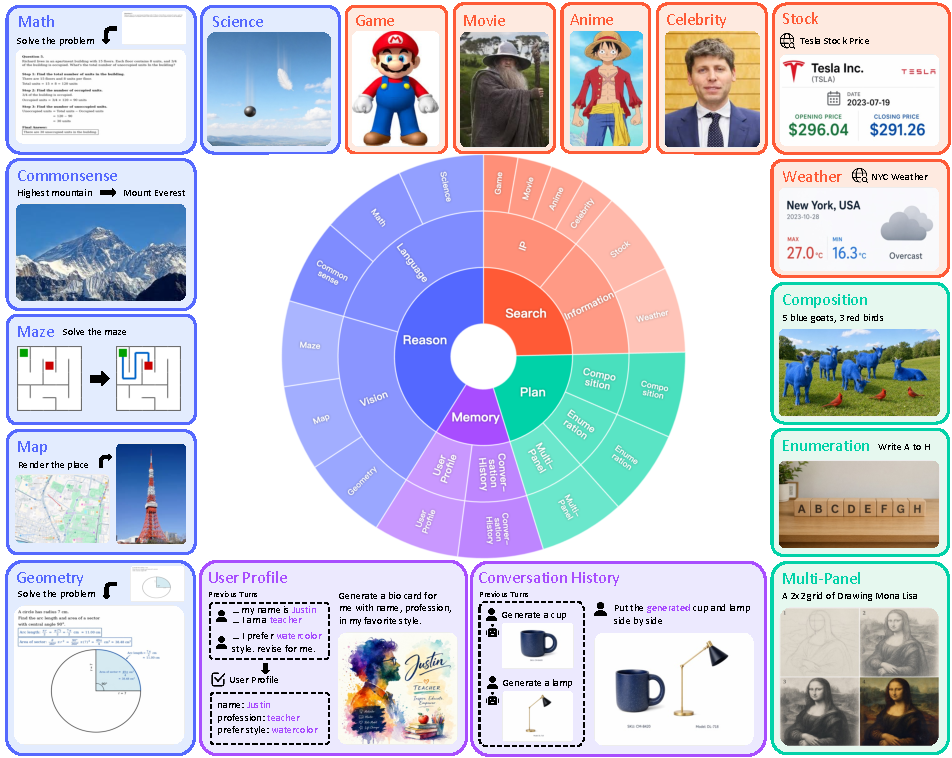
\includegraphics[width=\linewidth]{pics/qwen_image_agent_data.pdf}
    \caption{Overview of IA-Bench. IA-Bench covers 4 tasks, 17 subtasks, 730 instances and 1801 evaluation checklist items, providing a comprehensive evaluation of agentic image generation capabilities.}
    \label{fig:bench}
\end{figure*}

\subsection{Motivation and Overview}

Existing benchmarks for image generation mainly focus on rendering-oriented abilities, such as instruction following, visual fidelity, and aesthetic quality. However, real-world image generation often involves challenges beyond rendering alone: user requests may be underspecified, require external knowledge, demand multi-step decomposition, or depend on prior context. Addressing such requests requires models to infer implicit constraints, reason over intermediate decisions, retrieve relevant information, and maintain consistency across turns. These capabilities remain insufficiently studied in existing benchmarks, despite being particularly important for agentic image generation.

To address this gap, we introduce \textbf{Image Agent Bench (IA-Bench)}, a benchmark designed to evaluate the agentic capabilities involved in image generation. As illustrated in Figure~\ref{fig:bench}, IA-Bench covers four core capabilities: \textbf{Plan}, \textbf{Reason}, \textbf{Search}, and \textbf{Memory}. The benchmark consists of \emph{4 tasks, 17 subtasks, 730 instances and 1801 evaluation checklist items}. Together, they provide a structured evaluation framework for image generation systems across planning, reasoning, search, and memory dimensions.

\paragraph{Planning-Driven Tasks}
Planning-driven tasks evaluate whether a model can decompose a high-level goal into concrete visual arrangements and execute them in the final image. As illustrated in Figure~\ref{fig:bench}, this category includes tasks such as \textbf{Composition}, \textbf{Enumeration}, and \textbf{Multi-Panel}. These tasks require the model to explicitly organize multiple objects, satisfy counting constraints, and place visual elements into structured layouts. For example, a composition task may ask the model to place a specified number of objects with different attributes into a coherent scene, while a multi-panel task may require generating a grid of images that jointly satisfy a higher-level instruction. Such tasks emphasize deliberate planning over purely local rendering quality.

\paragraph{Reasoning-Driven Tasks}
Reasoning-driven tasks assess whether a model can infer latent constraints before generation and correctly ground the inferred result into the image. This category includes \textbf{Math}, \textbf{Science}, \textbf{Commonsense}, \textbf{Maze}, \textbf{Map}, and \textbf{Geometry}. These tasks involve three major types of reasoning: logical reasoning, commonsense reasoning, and visual reasoning. For example, a model may need to solve a math problem, infer the correct target from commonsense knowledge, or identify a valid path in a maze before rendering the final image. Unlike standard rendering tasks, success in this category depends on whether the model can first derive the correct intermediate conclusion and then faithfully express it in visual form.

\paragraph{Search-Driven Tasks}
Search-driven tasks assess whether a model can retrieve or ground external world knowledge that is not fully specified in the prompt. In IA-Bench, this category covers two major sources of knowledge: \textbf{IP}-related entities and \textbf{Information}. The \textbf{IP} branch includes tasks such as \textbf{Game}, \textbf{Movie}, \textbf{Anime}, and \textbf{Celebrity}, where the model must identify or accurately render well-known characters or people from cultural knowledge. The \textbf{Information} branch includes \textbf{Stock} and \textbf{Weather}, which require grounding up-to-date or structured real-world information into images. These tasks test whether image agents can go beyond prompt-local semantics and leverage retrieval or world knowledge to produce contextually correct outputs.

\paragraph{Memory-Driven Tasks}
Memory-driven tasks evaluate whether a model can preserve and reuse context across turns. This capability is essential for interactive image agents that must remain consistent with user preferences and prior dialogue history. IA-Bench includes \textbf{User Profile} and \textbf{Conversation History} task families. In user-profile tasks, the model must remember persistent user attributes, such as identity, profession, or preferred visual style, and incorporate them into later generations. In conversation-history tasks, the model must integrate previously generated content or earlier instructions into subsequent outputs, ensuring cross-turn consistency and correct composition. These tasks explicitly test whether the model can maintain coherent long-range context rather than treating each generation request independently.

\subsection{Benchmark Construction}

IA-Bench is constructed through careful human annotation with explicit attention to both quality and difficulty. During prompt collection, we filter out instances that can be solved by memorization or pretrained visual priors rather than the intended capability. For example, in IP-related tasks, we exclude highly iconic characters that text-to-image models can often generate correctly without external search. For each task, we further verify feasibility and minimize ambiguity in evaluation.

For checklist construction, annotators first use LLMs to generate candidates, which are then manually reviewed and refined to ensure that each item is correct and necessary. For memory-oriented tasks, we further design dynamic evaluation checklists, as the reference may be determined by images generated in earlier interaction turns rather than a static target.

\subsection{Evaluation Criterion}

To enable objective and fine-grained evaluation, we adopt a checklist-based evaluation protocol. For each test instance $i$, let $I^{i}_{\mathrm{gen}}$ denote the generated image and $\mathcal{C}^{i} = \{c^{i}_{j}\}_{j=1}^{K_i}$ denote its associated checklist, where each item corresponds to a required visual condition. We use a VLM to determine whether the generated image satisfies each checklist item. We report two complementary metrics:

\paragraph{Pass Rate (PR)}
Pass rate measures strict task success. An instance is considered successful only when all checklist items are satisfied:
\[
\mathrm{PR} = \frac{1}{N}\sum_{i=1}^{N}\prod_{j=1}^{K_i} \mathrm{VLM}(I^{i}_{\mathrm{gen}}, c^{i}_{j}).
\]

\paragraph{Checklist Accuracy (CA)}
Checklist accuracy measures the average proportion of checklist items satisfied by the generated image:
\[
\mathrm{CA} = \frac{1}{N}\sum_{i=1}^{N}\left(\frac{1}{K_i}\sum_{j=1}^{K_i} \mathrm{VLM}(I^{i}_{\mathrm{gen}}, c^{i}_{j})\right).
\]

Pass rate reflects strict end-to-end completion under all required constraints, whereas Checklist accuracy captures partial compliance in multi-constraint generation settings. Together, they characterize both holistic completion and partial fulfillment.

\paragraph{Image Agent score (IA-score)}
To summarize overall agent performance across different capability dimensions, we further report \textbf{IA-score}, a weighted aggregate score over the four core dimensions in IA-Bench: \textit{Plan}, \textit{Reason}, \textit{Search}, and \textit{Memory}. Specifically, IA-score is defined as
\[
\mathrm{IA\text{-}score} = 0.3 \times \mathrm{Plan} + 0.3 \times \mathrm{Reason} + 0.3 \times \mathrm{Search} + 0.1 \times \mathrm{Memory}.
\]
Here, \textit{Plan}, \textit{Reason}, \textit{Search}, and \textit{Memory} denote the micro average evaluation scores for their respective dimensions. We assign higher weights to \textit{Plan}, \textit{Reason}, and \textit{Search}, as these dimensions capture the core capabilities required for real-world image-agent tasks, while \textit{Memory} is included as a complementary factor for measuring cross-step consistency and context retention.
